\documentclass[../ana1.tex]{subfiles}
\begin{document}
\setcounter{section}{12}

\section{Konvergente Reihen, Teil 2}
Situation: \( {(a_n)}_n \) Folge in \( \R^d \) oder \( \C \).\\
Reihe \( \sum_{n=1}^\infty a_n \): geg.\ Folge Partialsummen:
\[ S_n := \sum_{j=1}^n a_j \]
Existiert \( \limes{n} S_n \), so ist der Wert von \( \sum_{n=1}^\infty a_n := \limes{n} S_n = \limes{n} \sum_{j=1}^n a_j. \)
\begin{satz}[Cauchykriterium]
    Eine Reihe \( \sum_{n=1}^\infty a_n \) in \( \R^d \) oder \( \C \) konvergiert
    \[ \Leftrightarrow \, \forall \, \varepsilon > 0 \,\exists \, K\in\N: \left| \sum_{j=n+1}^m a_j \right| < \varepsilon \,\forall \, m>n\geq K. \]
    \[ \Leftrightarrow \, \forall \, \varepsilon > 0 \,\exists \, K\in\N: \left| \sum_{j=n+1}^{n+p} a_j \right| < \varepsilon \,\forall \, n\geq K, p\in\N. \]
\end{satz}
\begin{bew}
    \[ \sum_{n=1}^\infty a_n \text{ konv. } \Leftrightarrow S_n := \sum_{j=1}^n a_j, {(S_n)}_n \text{ konvergiert.} \]
    \[ \overset{\text{Cauchy Folgen}}{\Leftrightarrow} {(S_n)}_n \text{ ist Cauchyfolge.} \]
    \[ \Leftrightarrow \,\forall \, \varepsilon > 0 \,\exists \, K\in\N: |\underbrace{S_m - S_n}_{=\sum_{j=n+1}^m a_j}| < \varepsilon \,\forall \, m>n\geq K \]
    \[ \Leftrightarrow \,\forall \, \varepsilon > 0 \,\exists \, K\in\N: \left| \sum_{j=n+1}^m a_j \right| < \varepsilon \,\forall \, m>n\geq K. \]
\end{bew}
\begin{bem}
    \[ \sum_n a_n \text{ konvergiert } \Rightarrow {(a_n)}_n \text{ ist Nullfolge. } a_n \rightarrow 0 \quad n\rightarrow \infty. \]
\end{bem}
\begin{defi}
    Eine Reihe \( \sum_{n=1}^\infty a_n, a_n\in\R^d \) heißt absolut konvergent, falls
    \[ \sum_{n=1}^\infty |a_n| \text{ konvergiert, d.\ h.\ } \sum_{n=1}^{\infty} |a_n| < \infty. \]
\end{defi}
\begin{satz}[absolute Konvergenz \(\Rightarrow \) Konvergenz]
    Falls \( \sum_n a_n, a_n\in\R^d,\C \), absolut konvergent ist, dann konvergiert sie und
    \[ \left| \sum_{n=1}^\infty a_n \right| \leq \sum_{n=1}^\infty |a_j|. \]
\end{satz}
\begin{bew}
    \( \sum_n a_n \) absolut konvergent \( \Leftrightarrow \sum_n |a_n| \) konvergiert.
    \[ \overset{\text{Satz 1}}{\Leftrightarrow} \,\forall \, \varepsilon > 0 \,\exists \, K\in\N: \sum_{j=n+1}^m |a_j| < \varepsilon \,\forall \, m>n\geq K. \]
    \[ \Rightarrow \left| \sum_{j=n+1}^m a_j \right| \leq \sum_{j=n+1}^m |a_j| < \varepsilon \,\forall \, m>n\geq K \]
    \[ \Rightarrow \sum_n a_n \text{ konvergiert.} \]
    Sei \( L \in\N \). 
    \[ \left| \sum_{n=1}^L a_n \right| \leq \sum_{n=1}^L |a_n| \leq \sum_{n=1}^\infty |a_n| < \infty \]
    \( \Rightarrow \abs{\sum_{n=1}^\infty a_n} \leq \sum_{n=1}^\infty \abs{a_n} \).
\end{bew}
\begin{defi}[Umordnung]
    Seien \( \sum_{n=1}^\infty a_n, \sum_{b=1}^\infty b_n \) Reihen in \( \R^d \). \( \sum_{n=1}^\infty b_n \) ist eine Umordnung von \( \sum_{n=1}^\infty a_n \), falls eine bijektive Abbildung \( \sigma:\N\rightarrow\N \) existiert mit
    \[ b_n = a_{\sigma(n)} \,\forall \, n\in\N. \]
\end{defi}
\begin{bem}
    Analog für \( \sum_{n=0}^\infty a_n, \sum_{n=0}^\infty b_n. \sigma: \N_0 \rightarrow \N_0 \) bijektiv.
\end{bem}
\begin{satz}[Umordnungssatz]
    Sei \( \sum_n a_n \) eine absolut konvergente Reihe. Dann konvergiert jede Umordnung gegen denselben Wert.
\end{satz}
\begin{bew}
    Sei \( \sigma : \N\rightarrow\N \) bijektiv. \( b_n := a_{\sigma(n)} \).
    \[ S_n = \sum_{j=1}^n a_j, \quad t_n := \sum_{j=1}^n b_j = \sum_{j=1}^n a_{\sigma(j)}. \]
    Wissen: \( \sum_{j=1}^\infty |a_j| < \infty, S = \limes{n} S_n \) existiert.
    Müssen zeigen: \( \limes{n} t_n = S \) (es reicht \( S_n - t_n \rightarrow 0, n\rightarrow\infty \).)
    Cauchykriterium: 
    \[ \forall \, \varepsilon > 0 \, \exists K\in\N: \sum_{j=n+1}^{n+p} |a_j| < \varepsilon \,\forall \, n\geq K, p\in\N. (*) \]
    \[ S_n - t_n = \sum_{j=1}^n a_j - \sum_{j=1}^n a_{\sigma(j)} \]
    \( \sigma : \N\rightarrow\N \) ist bijektiv. Wähle \( N\in\N, N\geq K \) so, dass
    \[ \{ a_1, a_2, \ldots, a_K \} \subset \{ a_{\sigma(1)}, a_{\sigma(2)}, \ldots, a_{\sigma(N)} \} \]
    \( \Rightarrow \) ist \( n\geq K \):
    \[ S_n - t_n = \sum_{j=1}^n a_j - \sum_{j=1}^n a_{\sigma(j)} = \sum_{1\leq j \leq n} a_{\sigma(j)} \text{ (mit } \sigma(j) > K\text{)} \]
    \[ |S_n - t_n| = \left| \sum_{1\leq j \leq n} a_{\sigma(j)} \right| \leq \sum_{1\leq j \leq n} | a_{\sigma(j)} | \leq \sum_{l>K} |a_l| \overset{(*)}{\leq}\varepsilon \]
    und somit auch \( S - t_n = (S-S_n) + (S_n - t_n) \rightarrow 0 + 0 = 0 \Rightarrow t_n \rightarrow S \).
\end{bew}
\begin{bem}
    Eine Reihe \( \sum_n a_n \) heißt unbedingt konvergent, falls wenn jede Umordnung \( \sum_n b_n \) ebenfalls fonvergiert und denselben Grenzwert besitzt. Andernfalls heißt \( \sum_n a_n \) bedingt konvergent.
\end{bem}
\begin{satz*}[Dirichlet 1837]
    \[ \sum_n a_n, a_n \in\R^d \text{ ist unbedingt konvergent } \Leftrightarrow \sum_n a_n \text{ ist absolut konvergent.} \]
\end{satz*}
\begin{bew}
    Hildebrandt: Analysis 1.
\end{bew}
\begin{satz*}[Riemann]
    Sei \( \sum_n a_n, a_n \in\R \) eine bedingt konvergente Reihe. Dann existiert zu jeder Zahl \( c\in\R \) eine Umordnung \( \sum_n b_n \) von \( \sum_n a_n \) mit \( \sum_{n=1}^\infty b_n = c \)
\end{satz*}
\begin{bspe}\leavevmode \\
    Mangold/Knopp: Einführung in die höhere Mathematik Band 2.\\
    Courent: \gqq{Vorlesungen} S. 328/329
    \[ \sum_{n=1}^\infty {(-1)}^{n+1} \frac{1}{n}. \]
\end{bspe}
\begin{bem}
    \( a\in\R, a_+ := \max(a,0) \geq 0, a_- := -\min(a,0)\geq 0 \).\\
    \( a = a_+ - a_- \quad |a| = a_+ + a_- \).
    \[ \sum_n |a_n| = \sum_n \left( {(a_n)}_+ + {(a_n)}_- \right) = \sum_n {(a_n)}_+ + \sum_n {(a_n)}_- \]
    \[ \Rightarrow \sum_n a_n \text{ bedingt konvergent} \Rightarrow \sum_n {(a_n)}_+ = +\infty = \sum_n {(a_n)}_- \]
\end{bem}
\begin{satz}[Test für absolute Konvergenz]
    Gilt eine der folgenden Bedingungen, so ist \( \sum_n a_n \) absolut konvergent.
    \begin{enumerate}
        \item Majorantenkriterium: \( |a_n| \leq c_n \) für fast alle \(n\) und \( \sum_n c_n < \infty \)
        \item Quotientenkriterium: \( \exists\, \theta \in [0,1) \) mit \( \frac{|a_{n+1}|}{|a_n|} \leq \theta \) für fast alle \(n\), \(a_n \neq 0\) für fast alle \(n\)
        \item Wurzelkriterium: \( \exists \, \theta \in [0,1) \sqrt[n]{|a_n|} \leq \theta \) für fast alle \(n\)
    \end{enumerate}
    Umgekehrt ist \( \sum_n a_n \) divergent, falls \( \frac{|a_{n+1}|}{|a_n|} \geq 1 \) für fast alle \(n\) oder \( \sqrt[n]{|a_n|} \geq 1 \) für fast alle \(n\)
\end{satz}
\begin{bew}\leavevmode
    \begin{enumerate}
        \item \( 0 \leq c_n, |a_n| \leq c_n \) für fast alle \( n, n\geq K\)
        \[ \Rightarrow \sum_{n=K}^{\infty} |a_n| \leq \sum_{n=K}^\infty c_n < \infty \Rightarrow \sum_{n=0}^\infty a_n \text{ absolut konvergent.} \]
        \item \( \exists \, K\in\N: \frac{|a_{n+1}|}{|a_n|} \leq \theta < 1 \, n\geq K. \)
        \[ |a_n| \leq \theta |a_{n-1}| \overset{\text{induktiv}}{\leq} \cdots \leq \theta^{n-K}|a_K| =: c_n. \]
        \[ \text{geom. Reihe: } \sum_{n=K}^\infty c_n = \sum_{n=K}^\infty \theta^{n-K}|a_K| = |a_K| \sum_{n=0}^\infty \theta^n = \frac{|a_K|}{1-\theta} < \infty. \]
        \( \Rightarrow \) 1.\ ist anwendbar. 
        \item \[ \sqrt[n]{|a_n|} \leq G \;\forall \; n\geq K \Rightarrow |a_n| \leq \theta^n \;\forall \; n\geq K \Rightarrow c_n = \theta^n \Rightarrow \sum_n c_n < \infty \]
        \( 0 \leq \theta < 1 \Rightarrow \) 1.\ anwendbar.\\
        Umgekehrt ist \( \frac{|a_{n+1}|}{|a_n|} \geq 1 \;\forall \; n\geq K \) \\
        \( \Rightarrow |a_n| \geq |a_{n-1}| \geq \cdots \geq |a_K| \) \\
        \( a_n \) ist keine Nullfolge \( \Rightarrow \sum_n a_n \) divergent.\\
        Ähnlich bei \( \sqrt[n]{|a_n|} \geq 1 \Rightarrow |a_n| \geq 1^n = 1 \)
    \end{enumerate}
\end{bew}
\begin{satz}[Cauchyprodukt]
    \( a_n, b_n \in\C \). Die Reihen \( \sum_{n=0}^\infty a_n, \sum_{n=0}^\infty b_n \) seien absolut konvergent.\\
    Dann ist auch \( \sum_{n=0}^\infty c_n \) mit 
    \[ c_n := \sum_{k+l=n} a_k b_l = \sum_{k=0}^n a_k b_{n-k} \]
    absolut konvergent und \( \sum_n c_n = ( \sum_{k=0} a_k )( \sum_{l=0} b_l ) \) \\
    und ist \(\tau \colon \; \N_0 \rightarrow \N_0 \times \N_0, n \mapsto \tau(n) = (\tau_1(n), \tau_2(n)) \) bijektiv
    \( p_n := a_{\tau_1(n)} \cdot b_{\tau_2(n)} \rightarrow \sum_{n=0}^\infty p_n \) absolut konvergent \\
    und \( \sum_{n=0}^\infty p_n = \sum_{k=0}^\infty a_k \cdot \sum_{l=0}^\infty b_l \).
\end{satz}
Bild:\\
\begin{prosa}
    \begin{center}
        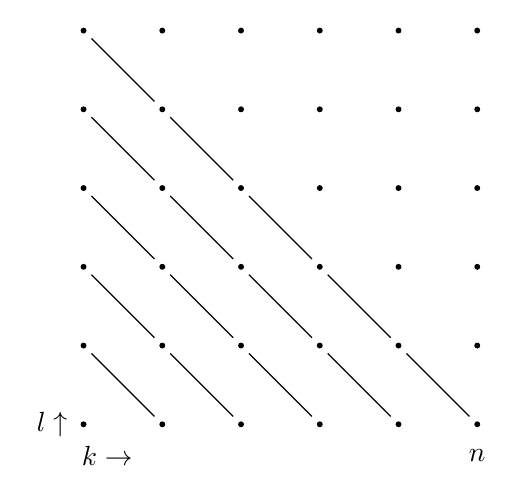
\begin{tikzpicture}
            \foreach \x in {0,...,5} {
                \foreach \y in {0,...,5} {
                    \draw[fill=black] (\x,\y) circle (0.03);
                }
            }
            \foreach \x in {1,...,5} {
                \foreach \y in {1,...,\x} {
                    \draw (5.1 - \x, \y - 0.1) -- (5.9 - \x, \y - 0.9);
                }
            }
            \draw (-0.4,0) node{\( l \uparrow \)};
            \draw (0.3,-0.4) node{\(k \rightarrow \)};
            \draw (5,-0.4) node{\(n\)};
        \end{tikzpicture}
    \end{center}
\end{prosa}
\begin{bew}
    Schritt 1: 
    \[ A_n := \sum_{k=0}^n \abs{a_k} \rightarrow \sum_{k=0}^\infty \abs{a_k} =: A < \infty \]
    \[ B_n := \sum_{l=0}^n \abs{b_l} \rightarrow \sum_{l=0}^\infty|b_l| =: B \]
    \( A_n \leq A_{n+1} \leq A \).
    \[ n\in\N \colon \; \sum_{j=0}^n \abs{c_j} \leq \sum_{j=0}^n \sum_{k+l=j} \abs{a_k b_l} = \sum_{\substack{0\leq k \\ l\leq n \\ k+l\leq n}} \abs{a_k}\abs{b_l} \]
    \[ \leq \sum_{\substack{0\leq k \\ l\leq n}} \abs{a_k} \abs{b_l} = \sum_{k=0}^n \sum_{l=0}^n \abs{a_k} \abs{b_l} \]
    \[ = \left( \sum_{k=0}^n \abs{a_k} \right) \cdot \left( \sum_{l=0}^n \abs{b_l} \right) = A_n \cdot B_n \leq A \cdot B < \infty \]
    \[ \text{d.\ h.\ } \forall \, n\in\N_0 \text{ ist } \sum_{j=0}^n \abs{c_n} \leq A \cdot B \overset{\text{Mon.\ Konv.}}{\Rightarrow} \sum_{j=0}^\infty \abs{c_j} \leq A \cdot B \]
    \( \Rightarrow \sum_{n=0}^\infty c_n \) ist absolut konvergent. \\
    Schritt 2:
    \[ S_n = \sum_{k=0}^n a_k \rightarrow S = \sum_{k=0}^\infty a_k, t_n := \sum_{l=0}^n b_l \rightarrow t = \sum_{l=0}^\infty b_l \]
    \[ S_n t_n - \sum_{j=0}^n c_j = \sum_{k=0}^n a_k \sum_{l=0}^n b_l - \sum_{j=0}^n c_j \]
    \[ = \sum_{\substack{0\leq k \\ l\leq n}} a_k b_l - \sum_{j=0}^n c_j = \sum_{\substack{0\leq k \leq n \\ 0\leq l \leq n}} a_k b_l - \sum_{j=0}^n \sum_{k+l=j} a_k b_l\]
    Man beachte:
    \[\sum_{j=0}^n \sum_{k+l=j} a_k b_l = \sum_{\substack{0\leq k \leq n \\ 0\leq l \leq n \\ k+l\leq n}} a_k b_l\]
    also:
    \[\sum_{\substack{0\leq k \leq n \\ 0\leq l \leq n}} a_k b_l - \sum_{j=0}^n \sum_{k+l=j} a_k b_l = \sum_{\substack{0\leq k \leq n \\ 0\leq l \leq n \\ k+l>n}} a_k b_l \]
    \[\Rightarrow \abs{ S_n t_n - \sum_{j=0}^n c_j } \leq \sum_{\substack{0\leq k\leq n \\ 0\leq l \leq n \\ k+l>n}} \abs{a_k}\abs{b_l}\]
    %Einschub
    Beachte: \( k,l \leq \frac{n}{2} \Rightarrow k + l \leq n \Rightarrow k + l > n \Rightarrow \max(k,l) > \frac{n}{2} \)
    \[ \leq \sum_{\substack{0\leq k\leq n \\ 0\leq l \leq n \\ \max(k,l) > \frac{n}{2}}} \abs{a_k b_l} \leq \sum_{\substack{0\leq k\leq n \\ 0\leq l \leq n \\ k > \frac{n}{2}}} \abs{a_k b_l} + \sum_{\substack{0\leq k\leq n \\ 0\leq l \leq n \\ l>\frac{n}{2}}} \abs{a_k b_l} \]
    \[ = \sum_{\frac{n}{2} < k \leq n} \sum_{l=0}^n \abs{a_k}\abs{b_l} + \sum_{k=0}^n \sum_{\frac{n}{2} < l \leq n} \abs{a_k b_l} \]
    \[ = \underbrace{\left( \sum_{\frac{n}{2} < k \leq n} \abs{a_k} \right)}_{\rightarrow 0 \text{(Cauchy-krit)}} \cdot \underbrace{\left( \sum_{l=0}^n \abs{b_l} \right)}_{=B_n < B} + \underbrace{\left( \sum_{k=0}^n \abs{a_k} \right)}_{=A_n \leq A} \cdot \underbrace{ \left( \sum_{\frac{n}{2} < l \leq n} \abs{b_l} \right) }_{\rightarrow 0, n\rightarrow\infty} \]
    \[ \rightarrow 0, n\rightarrow\infty \]
    \[ \Rightarrow \limes{n} \sum_{j=0}^n c_j = \limes{n} S_n t_n = S t = \left( \sum_{k=0}^\infty a_k \right) \left( \sum_{l=0}^\infty b_l \right) \]
    Schritt 3: \( \tau \colon \N_0 \rightarrow \N_0 \times \N_0, p_n = a_{\tau_1(n)} b_{\tau_2(n)} \) \\
    \( \sum_{j=0}^n \abs{p_j} = \ ? \)
    Geg. \(n\in\N \), wähle \( M\in\N_0 \) so, dass 
    \[ \{ \tau(0), \tau(1), \ldots, \tau(n) \} \subset \{ (k,l) \; \vert \; 0 \leq k \leq M, 0 \leq l \leq M \} \]
    \[ \Rightarrow \sum_{j=0}^n \abs{p_n} = \sum_{j=0}^n \abs{a_{\tau_1(n)} b_{\tau_2(j)}} \leq \sum_{\substack{0\leq k\leq M \\ 0 \leq l \leq M}} \abs{a_k b_l} = \sum_{k=0}^M \abs{a_k} \sum_{l=0}^M \abs{b_l} \] 
    \[ = A_M B_M \leq A \cdot B < \infty \]
    \[ \Rightarrow \sum_{j=0}^\infty p_j \text{ ist absolut konvergent.} \]
    Schritt 4: \( \tau : \N_0 \rightarrow \N_0 \times \N_0 \bijektiv \)
    \[ \Rightarrow \, \forall \, m\in\N_0 \, \exists \, n\in\N_0 : \{ (k,l) \; \vert \; 0\leq k\leq m, 0\leq l\leq m \} \subset \{ \tau(0), \tau(1), \ldots, \tau(n) \} \]
    \( \Rightarrow \) Wähle induktiv. 
    Bild: 
    %BILD
    \( n_0 < n_1 < n_2 < \cdots < n_m < n_{m+1} < \ldots \) mit 
    \[ \{ (k,l) \; \vert \; 0 \leq k, l \leq m \} \subset \{ \tau(0), tau(1), \ldots , \tau(n_m) \} \, \forall \, m\in\N_0 \]
    \[ \abs{ S_m t_m - \sum_{j=0}^{n_m} \underbrace{ a_{\tau_1(j)} b_{\tau_2(j)} }_{=p_j} } = \abs{ \sum_{\substack{0\leq j\leq n_m \\ \tau_1(j) > m \vee \tau_2(j) > m}} a_{\tau_1(j)} b_{\tau_2(j)} } \]
    \[ \leq \sum_{\substack{0\leq k \leq n_m \\ \tau_1(j) > m \vee \tau_2(j) > m}} \abs{a_{\tau_1(j)} b_{\tau_2(j)}} \]
    \[ L_m := \underset{0\leq j\leq n}{\max}(\max( \tau_1(j), \tau_2(j) ) ) \]
    \[ \leq \sum_{\substack{0\leq k \\ l\leq L_m \\ k > m \vee l > m}} \abs{a_k} \abs{b_l} = \sum_{\substack{0\leq k\leq L_m \\ m<l\leq L_m}} \abs{a_k}\abs{b_l} + \sum_{\substack{0\leq l \leq L_m \\ m<k\leq L_m}} \abs{a_k}\abs{b_l} \]
    \[ = \underbrace{\left( \sum_{k=0}^{L_m} \abs{a_k} \right)}_{\leq A_{L_m} \leq A} \cdot \underbrace{\left( \sum_{l=m+1}^{L_m} \abs{b_l} \right)}_{\leq \sum_{l=m+1}^\infty \abs{b_l} \rightarrow 0, m\rightarrow \infty} + \left( \sum_{k=m+1}^{L_m} \abs{a_k} \right) \cdot \left( \sum_{l=0}^{L_m} \abs{b_l} \right) \rightarrow 0, m\rightarrow\infty \]
    \[ U_n = \sum_{j=0}^n p_j, \Rightarrow \text{ Teilfolge } {(u_{n_m})}_m \text{ konvergiert gegen } S \cdot t. \]
    \[ n_0 < n_1 < n_2 < \cdots < n_m < n_{m+1} < \dots \]
    Aus Schritt 3: wir wissen, dass \( (u_n)_n \) eine konvergente Folge ist, \( \Rightarrow \limes{n} u_n = \limes{n} u_{n_m} = S \cdot t. \)
\end{bew}
\end{document}